\documentclass[11pt]{ctexart}

\usepackage{multicol}
%\usepackage{mwe}
\usepackage{subfigure}
\usepackage{mathtools}
\usepackage{graphicx}
\usepackage{amsmath}
\usepackage{mathrsfs}
\usepackage[top=0.5in,bottom=1in,left=1in,right=1in]{geometry}
\usepackage{pdflscape}
\usepackage{times}
\usepackage{bm}
%\usepackage{setspace}
\usepackage{color}
\usepackage{caption}
\usepackage{amsmath}
\usepackage{amssymb}
\usepackage{CJK}
%\usepackage[final]{pdfpages}
\usepackage{listings}
\usepackage{textcomp}
\usepackage{xcolor}
\usepackage{algorithm2e}

\usepackage{algorithmicx}
\usepackage{algpseudocode}
\usepackage{hyperref}

\hypersetup{hidelinks,
	colorlinks=true,
	allcolors=black,
	pdfstartview=Fit,
	breaklinks=true}

\pagestyle{plain}




\begin{document}

\title{第二周实习报告20220309}
\author{宋欣源}
\date{\today}

\maketitle % need full-width title

\CTEXsetup[format={\Large\bfseries}]{section}

\section{第一,综述}

下面对于这五天实习的工作做一个报告。首先解决的问题是将batch\_size变大1024.
我这周主要分成两个大的方向,CNN和RNN

\section{第一,CNN}
\subsection{综述}
在CNN领域,主要的思想是利用deepwise,普通CNN2d,和pointwise做特征提取。首先,我对各类CNN的基础性能进行了实验。

模型1:普通CNN2d
普通CNN2d要建立新的假象维度,把假象维度拆分成隐藏维度,假象维度只能是1,因为使用了假象维度,卷积核应该和特征数保持一致。(如果不一致,就要做下一层的CNN提取,目前先保持一致,采用卷积核大小为3)
\begin{itemize}
  \item [1)]
  CNN1d(1,50,3*3)
  \item [2)]
  maxpool1d+dropout
  \item [3)]
  每个时间取最后
  \item [4)]
  两层全连接层,中间加relu

\end{itemize}
结果: batch\_size 1024, batchIC = 0.041,
pnl图(7epoch):
\begin{figure}[!ht]
\begin{center}
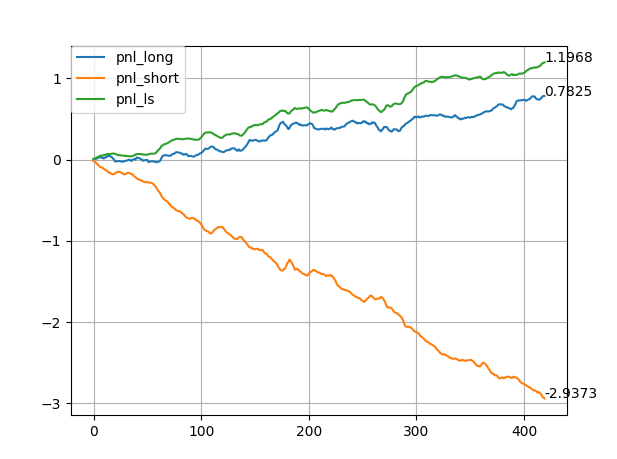
\includegraphics[width=0.5\textwidth]{4.PNG}
\end{center}
\caption{1layer CNN2d pnl figure}
\label{FIG.1}
\end{figure}

模型2:deepCNN2d
\begin{itemize}
  \item [1)]
  deepwise CNN2d(1024,1300,3*3, 1300)
  \item [2)]
  maxpool1d+dropout
  \item [3)]
  每个时间取最后和取时间平均都做尝试
  \item [4)]
  两层全连接层,中间加relu

\end{itemize}
结果: batch\_size 1024, batchIC = 0.047,
pnl图(7epoch):
\begin{figure}[!ht]
\begin{center}
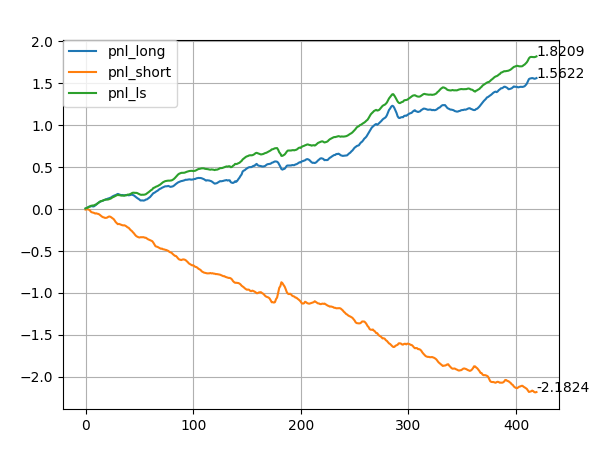
\includegraphics[width=0.5\textwidth]{5.PNG}
\end{center}
\caption{deep CNN2d pnl figure}
\label{FIG.2}
\end{figure}

模型3:pointCNN2d
\begin{itemize}
  \item [1)]
  deepwise CNN2d(1024,1300,3*3, 1300)
  \item [2)]
  maxpool1d+dropout
  \item [3)]
  pointwise CNN1d(T,1, 1)用cnn1d提取时间轴特征,时间轴提取到一
  \item [4)]
  两层全连接层,中间加relu

\end{itemize}
结果: batch\_size 1024, batchIC = 0.048,
pnl图(7epoch):
\begin{figure}[!ht]
\begin{center}
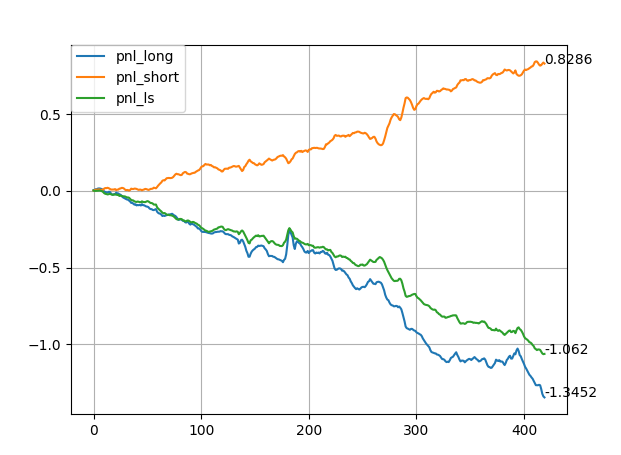
\includegraphics[width=0.5\textwidth]{1.PNG}
\end{center}
\caption{pointCNN2d pnl figure}
\label{FIG.3}
\end{figure}

\subsection{模型与实现}
经过上面的验证pointwise的效果并不很好,经过大量实验发现,pointwise适合时间序列提取特征,而CNN适合从特征轴和假象维度提取特征。很容易想到先用deepwise在特征上提取,再用pointwise在时间轴上提取时间特征。(原先的方法是在时间维度上取-1)

模型4:deepCNN2d+pointCNN2d
\begin{itemize}
  \item [0)]
  deepwise CNN2d
  \item [1)]
  pointwise CNN2d
  \item [2)]
  maxpool1d+dropout
  \item [3)]
  pointwise CNN2d(T,1, 1*1)用cnn1d提取时间轴特征,时间轴提取到一
  \item [4)]
  两层全连接层,中间加relu

\end{itemize}
结果: batch\_size 1024, batchIC = 0.047, pnl = 1.874
pnl图(7epoch)
\begin{figure}[!ht]
\begin{center}
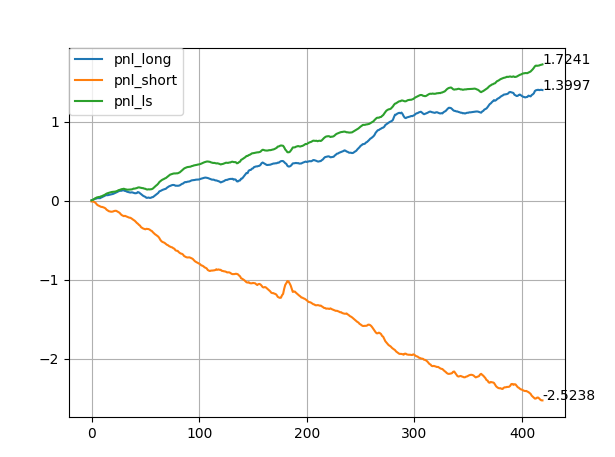
\includegraphics[width=0.5\textwidth]{3.PNG}
\end{center}
\caption{deepCNN+pointCNN pnl figure}
\label{FIG.4}
\end{figure}

上面deepwise的做法是生成了假象的1个维度,这样在新的T*3的平面上可以运用CNN2d.生成新的假象维度(F)。然后在(F*T)上运用新的CNN2d。反复运用。由于本来F的维度就是3,所以不能padding,得到新的一维,再squeeze掉这一维,剩下的维度保持和原来一直(N,T,F)然后用pointwise再时间轴上提取信息,用线性全连接层提取F特征信息。

模型5:deepCNN2d*2+pointCNN2d
每个卷积都用两层卷积来做,效果更好。
\begin{itemize}
  \item [0)]
  deepwise CNN2d
  \item [1)]
  pointwise CNN2d
  \item [2)]
  maxpool1d+dropout
  \item [3)]
  pointwise CNN2d(T,1, 1*1)用cnn1d提取时间轴特征,时间轴提取到一
  \item [4)]
  两层全连接层,中间加relu

\end{itemize}
结果: batch\_size 1024, batchIC = 0.047, pnl = 1.965

尝试了三层,四层,结果发现层数越多,效果越好,在此就不再赘述了。
另一个思路是普通的CNN,不是deepwise版本。普通的CNN2d在这个数据集上无法使用。(如果在FT平面上卷积,就必须将N维度展开,这显然是不可取的。如果在NF平面上卷积,就必须将T维度展开,这显然是不可取的。)所以只能用deepwise首先新增假象维度,形成(N,T,F1,F2)的形状。然后在(F1,F2)平面上ordinary CNN2d。另一种做法是将F1和F2进行view,本身这些特征都是统一时间统一截面的,所以不影响。

模型6 
\begin{itemize}
  \item [0)]
  deepwise CNN2d*2
  \item [1)]
  view
  \item [1)]
  pointwise CNN2d
  \item [2)]
  maxpool1d+dropout
  \item [3)]
  pointwise CNN2d(T,1, 1*1)用cnn1d提取时间轴特征,时间轴提取到一
  \item [4)]
  两层全连接层,中间加relu

\end{itemize}
结果: batch\_size 1024, batchIC = 0.057, pnl = 2.08
\begin{figure}[!ht]
\begin{center}
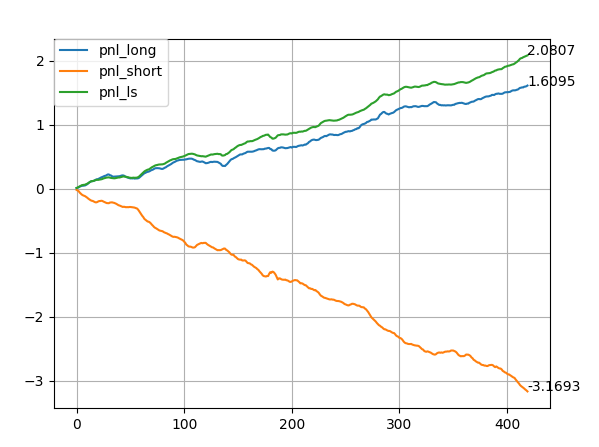
\includegraphics[width=0.5\textwidth]{ws.PNG}
\end{center}
\caption{deepCNN*2+pointCNN pnl figure}
\label{FIG.5}
\end{figure}

模型7 
\begin{itemize}
  \item [0)]
  deepwise CNN2d
  \item [1)]
  ordinaryCNN2d
  \item [1)]
  pointwise CNN2d
  \item [2)]
  maxpool1d+dropout
  \item [3)]
  pointwise CNN2d(T,1, 1*1)用cnn1d提取时间轴特征,时间轴提取到一
  \item [4)]
  两层全连接层,中间加relu
\end{itemize}
结果: batch\_size 1024, batchIC = 0.068, pnl = 2.25
\begin{figure}[!ht]
\begin{center}
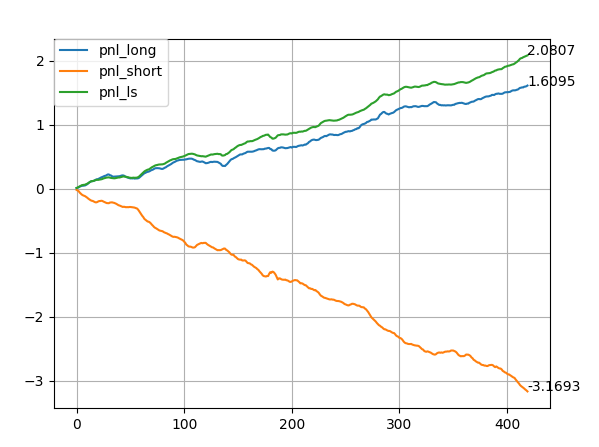
\includegraphics[width=0.5\textwidth]{ws.PNG}
\end{center}
\caption{deepCNN*2+pointCNN pnl figure}
\label{FIG.5}
\end{figure}

在进行到ordinary2d的时候,仍然可以采用deep wise的办法,将卷积核扩大到F2的数量,这样保证卷积出来的结果有一个维度,再squeeze掉就可以了。经过实验,发现没有ordinary2d的效果好。

模型8
\begin{itemize}
  \item [0)]
  deepwise CNN2d
  \item [1)]
  deepwise(kernel\_size = F2)
  \item [1)]
  pointwise CNN2d
  \item [2)]
  maxpool1d+dropout
  \item [3)]
  pointwise CNN2d(T,1, 1*1)用cnn1d提取时间轴特征,时间轴提取到一
  \item [4)]
  两层全连接层,中间加relu
\end{itemize}
结果: batch\_size 1024, batchIC = 0.064, pnl = 2.16

进行到这里,开始添加maxpool和avgpool层。经过实验,添加avgpool以后效果和原来很像,而添加max以后效果明显变差。IC下降到0.03,pnl下降到1.3,和普通层区别不大。需要进一步研究。

\subsection{改进思路}
\begin{itemize}
  \item [1)]
  从CNN的层数叠加,比如多层CNN2d(deepwise)叠加,已经发现层数越多效果越好,不如4,5,6暴力叠加。因为deepwise不操作时间序列,所以基本上没有时间信息损失,可以反复叠加。
  \item [2)]
  这些操作都是down操作,目的在于压缩维度。可以添加CNN进行扩展维度up,可以将压缩的维度重新扩展,再压缩,最后的曲线特征明显而且平滑。
\end{itemize}

\section{RNN的研究}
\subsection{综述}
RNN的研究主要是四个方面。研究cell和循环的写法,自创cell,在cell里运用多个时间节点,不同cell的串并联,以及其他复杂跨cell操作。

首先利已有的RNN模块进行实(多层lstm,多层gru,lstm+gru)等,pnl大多在1.6-1.9之间。然后研究了rnncell的写法,其中有几个坑,都已经完美解决(梯度迭代,计算图清除,保存hiddenstate)

\subsection{LSTMC}
lstm的cell公式如下:

\begin{equation}
\begin{split}
    i_t &= \sigma (W_{x i} x_t + W_{H i} h_{t-1} + b_i)\\
    f_t &= \sigma (W_{x f} x_t + W_{H f} h_{t-1} + b_f)\\
    c_t &= f_t \odot c_{t-1} + i_t \odot \tanh (W_{x c} x_t + W_{H c} h_{t-1} + c_i)\\
    o_t &= \sigma (W_{x o} x_t + W_{H o} h_{t-1} + b_o)\\
    h_t &= o_t \odot \tanh(c_t)
\end{split}
\end{equation}

那么很容易做修改,相当于将cell state也作为hidden state 影响每一个输出结果,为LSTMC cell
\begin{equation}
\begin{split}
    i_t &= \sigma (W_{x i} x_t + W_{H i} h_{t-1} + W_{c i} c_{t-1} + b_i)\\
    f_t &= \sigma (W_{x f} x_t + W_{H f} h_{t-1} + W_{c f} c_{t-1} +b_f)\\
    c_t &= f_t \odot c_{t-1} + i_t \odot \tanh (W_{x c} x_t + W_{H c} h_{t-1} + W_{c c} c_{t-1} +b_c)\\
    o_t &= \sigma (W_{x o} x_t + W_{H o} h_{t-1} + W_{c o} c_{t-1} +b_o)\\
    h_t &= o_t \odot \tanh(c_t)
\end{split}
\end{equation}
经过简单的循环实验,发现比lstm的性能提高了很多,IC达到0.68,pnl达到2.3
\begin{figure}[!ht]
\begin{center}
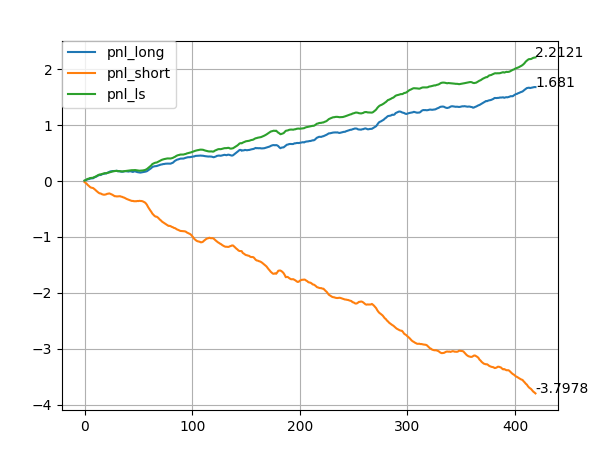
\includegraphics[width=0.5\textwidth]{ww.PNG}
\end{center}
\caption{LSTMC simplenet pnl figure}
\label{FIG.6}
\end{figure}

那么很容易做修改,将$x_{t-1}, x_{t-2},...$也作为每个门的 输入, 影响每一个输出结果,为pasttime cell
\begin{equation}
\begin{split}
    i_t &= \sigma (W_{x_t i} x_t + W_{x_{t-1} i} x_{t-1} +W_{H i} h_{t-1} + b_i)\\
    f_t &= \sigma (W_{x_t f} x_t + W_{x_{t-1} f} x_{t-1} +W_{H f} h_{t-1} + b_f)\\
    c_t &= f_t \odot c_{t-1} + i_t \odot \tanh (W_{x_t c} x_t + W_{x_{t-1} c} x_{t-1} +W_{H c} h_{t-1} + b_c)\\
    o_t &= \sigma (W_{x_t o} x_t + W_{x_{t-1} o} x_{t-1} +W_{H o} h_{t-1} + b_o)\\
    h_t &= o_t \odot \tanh(c_t)
\end{split}
\end{equation}
这种改法没有上面的效果好,但是我只尝试了运用前一天的数据结果。可以尝试多用几天,用平均,和上面结合的办法提高效果,后面继续尝试。


那么很容易做修改,将记忆门的相反数作为遗忘门, 有如下结果:
\begin{equation}
\begin{split}
    f_t &= \sigma (W_{x_t f} +W_{H f} h_{t-1} + b_f)\\
    c_t &= f_t \odot c_{t-1} + (1-f_t) \odot \tanh (W_{x_t c} x_t +W_{H c} h_{t-1} + b_c)\\
    o_t &= \sigma (W_{x_t o} x_t +W_{H o} h_{t-1} + b_o)\\
    h_t &= o_t \odot \tanh(c_t)
\end{split}
\end{equation}
这种改法没有上面的效果好,多一个门多一层参数,网络不改的话效果相对差一些。可以尝试上面结合的办法提高效果,后面继续尝试。


注意:RNNcell的设计存在一大困难。由于梯度经过循环推送,最后实际上求导次数可能达到上万次,很容易出现梯度消失和梯度爆炸,总结出几个暂时性结论,用于实验。
\begin{itemize}
  \item [0)]
  所有中间的cell,阶数必须相等,不相等分分钟梯度消失。
  \item [1)]
  在特定的时候必须使用特定的激活函数,sigmoid,tanh,relu,用错直接梯度爆炸或爆炸
  \item [1)]
  如果进入cell的数据不止一个,必须保证所有进入的数据结束相等,不相等直接梯度爆炸
\end{itemize}

\subsection{PASScell}
passcell是我自己研究出来的两种cell,单独的cell网络效果还可以,还需要进一步研究。
\begin{equation}
\begin{split}
    i_t &= \sigma (W_{x i} x_t + W_{H i} h_{t-1} + b_i)\\
    f_t &= \sigma (W_{x f} x_t + W_{H f} h_{t-1} + b_f)\\
    o_t &= \sigma (W_{x o} x_t + W_{H o} h_{t-1} + b_o)\\
    g_t &= \sigma (W_{x g} x_t + W_{H g} h_{t-1} + b_g)\\
    output_t &= f_t * output_{t-1} - i_t * \tanh(g_t)\\
    h_t &= o_t * \tanh(output_{t-1})
\end{split}
\end{equation}
\begin{figure}[!ht]
\begin{center}
\includegraphics[width=0.8\textwidth]{sxy\_rnn1.PNG}
\end{center}
\caption{pass1cell simplenet structure}
\label{FIG.7}
\end{figure}
表现如下
\begin{figure}[!ht]
\begin{center}
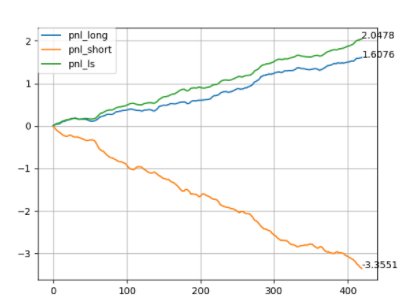
\includegraphics[width=0.5\textwidth]{wde.PNG}
\end{center}
\caption{pass1cell simplenet pnl figure}
\label{FIG.8}
\end{figure}

问题在于,为什么h不能链接传递矩阵,而是连接输出呢。答案,连接传递门造成阶数不相等,直接梯度爆炸。暂时还没有尝试接传递门再加新门的结果。

\subsection{PASScel2}
passcel2是我自己研究出来的两种cell,单独的cell网络效果还可以,还需要进一步研究。

\begin{equation}
\begin{split}
    h_t &= \tanh(W_{f input} input_{t-1} + W_{f output_{t-1}} output_{t-1} + W_{f h} h_{t-1})\\
    output_t &= \sigma(W_{z z} z_t)\\
    z_t &= \sigma(W_{cat} [x_t, u_t])
\end{split}
\end{equation}

思路在于,将输入和cellstate共同作为输入循环的更新cellstate,保证梯度不爆炸。
\begin{figure}[!ht]
\begin{center}
\includegraphics[width=0.8\textwidth]{sxy\_rnn3.PNG}
\end{center}
\caption{pass2cell simplenet structure}
\label{FIG.9}
\end{figure}
表现如下
\begin{figure}[!ht]
\begin{center}
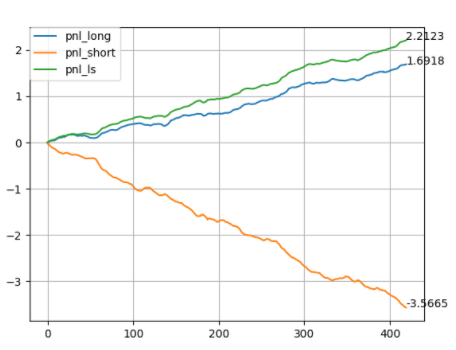
\includegraphics[width=0.5\textwidth]{wwd.PNG}
\end{center}
\caption{pass12ell simplenet pnl figure}
\label{FIG.10}
\end{figure}

试了很久,终于不爆炸了,门控rnn还需要进一步研究。

尝试了各类cell连接全连接层,效果不好,以后不做全连接层。

\subsection{cell并联}
构建好了各类的cell,就可以将cell进行串并联,结构如下:
\begin{figure}[!ht]
\begin{center}
\includegraphics[width=0.8\textwidth]{sxy\_rnn2.PNG}
\end{center}
\caption{cell的串并联 figure}
\label{FIG.11}
\end{figure}
按照上面的方式并联,结果如下:
\begin{figure}[!ht]
\begin{center}
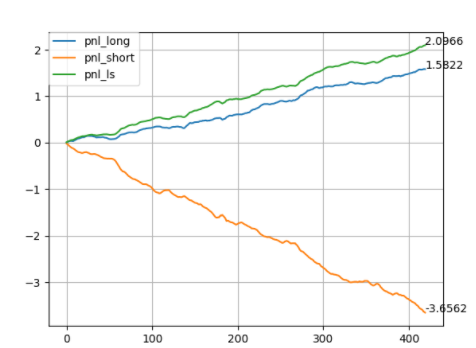
\includegraphics[width=0.5\textwidth]{wws.PNG}
\end{center}
\caption{cell的串并联 figure}
\label{FIG.12}
\end{figure}
cell可以进行大量的串并联,继续研究。


\section{总结}
我打算在CNN领域进行深度挖掘,把deeplab,bottleneck等CNN常用模型进行组合尝试,用自己的理解构造一些复杂CNN累积处理神经网络。
我打算在RNNcell领域进行深度挖掘,自己设计一些有用的cell,进行cell的串并联,用自己的理解构造一些复杂门神经网络。

\end{document} 